
% Q15
\question If the arc length and the area of a sector are $8\pi\text{ cm}$ and $80\pi\text{ cm}^2$ respectively, then the angle of the sector is
\begin{choices}
    \choice $36^\circ$ .
    \choice $45^\circ$ .
    \choice $60^\circ$ .
    \correctchoice $72^\circ$ .
\end{choices}
\begin{solution}
Let $r\text{ cm}$ and $\theta$ be the radius and the angle of the sector respectively.
\[ \text{Area} = \frac{1}{2}r\ell \implies 80\pi = \frac{1}{2}r(8\pi) \implies r = 20 \]
From the arc length:
\[ 2\pi(20) \times \frac{\theta}{360^\circ} = 8\pi \implies \theta = 72^\circ \quad \text{(D)} \]
\end{solution}

% Q16
\question The ratio of the height of a right circular cylinder to the height of a right circular cone is $32 : 15$ while the ratio of the volume of the circular cylinder to the volume of the circular cone is $10 : 9$ . If the base radius of the circular cylinder is $25\text{ cm}$ , then the base radius of the circular cone is
\begin{choices}
    \choice $20\text{ cm}$ .
    \choice $24\text{ cm}$ .
    \choice $48\text{ cm}$ .
    \correctchoice $60\text{ cm}$ .
\end{choices}
\begin{solution}
Let $r\text{ cm}$ be the base radius of the circular cone.
\[ \frac{\pi(25)^2(32)}{\frac{1}{3}\pi r^2(15)} = \frac{10}{9} \implies \frac{625 \times 32}{5r^2} = \frac{10}{9} \implies r^2 = 3600 \implies r = 60 \quad \text{(D)} \]
\end{solution}

% Q17
\question In the figure, $ABCD$ is a square. Let $M$ be the mid-point of $BC$ . $E$ is a point lying on $AD$ such that $AE : ED = 3 : 1$ . $F$ is a point lying on $BC$ produced such that $EF$ // $AM$ . $CD$ and $EF$ intersect at the point $G$ while $AM$ and $BG$ intersect at the point $H$ . If the area of $\triangle BMH$ is $4\text{ cm}^2$ , then the area of the trapezium $AEGH$ is

\begin{minipage}{0.45\textwidth}
\begin{choices}
    \choice $12\text{ cm}^2$ .
    \choice $33\text{ cm}^2$ .
    \correctchoice $39\text{ cm}^2$ .
    \choice $45\text{ cm}^2$ .
\end{choices}
\end{minipage}
\begin{minipage}{0.52\textwidth}
\centering
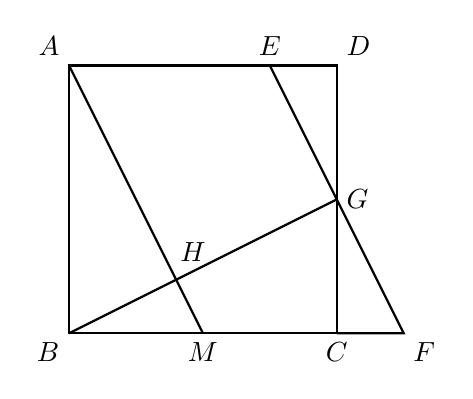
\begin{tikzpicture}[scale=0.85]
    \coordinate (B) at (0,0);
    \coordinate (C) at (4,0);
    \coordinate (D) at (4,4);
    \coordinate (A) at (0,4);
    \coordinate (M) at (2,0);
    \coordinate (E) at (3,4);
    \coordinate (F) at (5,0);
    \coordinate (G) at (4,2);
    \coordinate (H) at (1.6,0.8);
    \draw[thick] (A) -- (B) -- (C) -- (D) -- cycle;
    \draw[thick] (C) -- (F) -- (E);
    \draw[thick] (A) -- (M);
    \draw[thick] (B) -- (G);
    \node[above left] at (A) {$A$};
    \node[below left] at (B) {$B$};
    \node[below] at (M) {$M$};
    \node[below] at (C) {$C$};
    \node[below right] at (F) {$F$};
    \node[above right] at (D) {$D$};
    \node[above] at (E) {$E$};
    \node[right] at (G) {$G$};
    \node[above=10pt, right=-2pt] at (H) {$H$};
\end{tikzpicture}
\end{minipage}
\begin{solution}
Place $B$ at $(0,0)$ with square side length $4$: $A(0,4)$, $M(2,0)$, $E(3,4)$, $D(4,4)$. \\
Since $EF$ // $AM$ (slope $-2$) and $ED = 1$, $G$ is at $(4,2)$, the mid-point of $CD$. \\
By $\triangle ABM \cong \triangle BCG$, we have $AM \perp BG$, so $\triangle BMH \sim \triangle BMA$ with $BM : BA = 1 : 2$. \\
Since $\text{Area of } \triangle BMH = 4\text{ cm}^2$, $\text{Area of } \triangle ABH = 16\text{ cm}^2$ and $\text{Area of } \triangle ABM = 20\text{ cm}^2$, so $\text{Area of } ABCD = 80\text{ cm}^2$. \\
Then $\text{Area of } \triangle BCG = 20\text{ cm}^2$ and $\text{Area of } \triangle EDG = \frac{1}{2}\left(\frac{1}{4}\right)\left(\frac{1}{2}\right)(80) = 5\text{ cm}^2$. \\
Thus, $\text{Area of } AEGH = 80 - \text{Area}(\triangle ABH) - \text{Area}(\triangle BCG) - \text{Area}(\triangle EDG) = 80 - 16 - 20 - 5 = 39\text{ cm}^2$ (C).
\end{solution}